\chapter{细胞分化：骨骼肌细胞}\label{ch:b2:cell-differentiation}

你大腿肌肉中的一根\omterm{def:b2:cell-differentiation:myogenesis}{肌纤维}是一个单细胞，长三十厘米，
内含数百个细胞核，首尾相接地排满
收缩性杆状结构，排列极其规整，
在显微镜下呈现条纹。它最初是一群外观普通的细胞，
从\omterm{prop:b2:vertebrate-development:neurulation}{体节}中迁出、增殖、停止分裂、排成一列，
融合，并开启了数百个
此前从未使用过的基因。体内每个细胞都具有相同的基因组；\omterm{def:b2:cell-differentiation:myogenesis}{肌纤维}
即该基因组在某一特定\omterm{prop:b2:cell-differentiation:transcriptional}{转录因子}
被开启时所产生的结果。本章以骨骼肌细胞为例
讲解\emph{\omterm{def:b2:cell-differentiation:differentiation}{分化}}——细胞如何获得
并保持其特化的身份——骨骼肌细胞是一个很好的例子，
因为其主控开关已经明确，\omterm{def:b2:cell-differentiation:differentiation}{分化}步骤可以在培养皿中观察，
成熟细胞则是一台部件清晰可见的机器。

\section{什么是分化}

\begin{definition}[分化、决定、潜能]\label{def:b2:cell-differentiation:differentiation}
\index{分化}\index{决定}\index{干细胞}\index{潜能}
细胞表达某一细胞类型所特有的稳定基因模式
（从而决定其蛋白质、形态与功能）时，称其为\emph{已分化的}。
其命运已定，而分化尚未开始时，称其为\emph{已决定的}（或已定向的）；
例如\omterm{def:b2:cell-differentiation:myogenesis}{成肌细胞}：
外观像成纤维细胞，却只能产生肌肉。\emph{潜能}是
细胞仍能产生的类型范围：\emph{全能}的（受精卵与最初的\omterm{def:b2:vertebrate-development:egg}{卵裂}球，
能产生一切细胞，
包括\omterm{def:b2:mammal-reproduction:placenta}{胎盘}在内）、\emph{多能}的（\omterm{def:b2:mammal-reproduction:implantation}{内细胞团}，
能产生体内的每一种组织）、\emph{专能}的（血液或肌肉的干细胞，
只产生一种组织中的几类细胞），
\emph{单能}的。\emph{干细胞}是这样一类细胞：分裂时产生
一个与自身相同的子细胞，以及另一个将继续分化的子细胞，
从而在保持细胞库的同时为组织供应新细胞。
分化在多数情况下并不是基因的丢失，而是对基因的选择：
肌细胞核的基因组是完整的。
\end{definition}
\begin{proof}[证据]
格登（1962）将一只蝌蚪已\omterm{def:b2:cell-differentiation:differentiation}{分化}的
肠细胞的细胞核移入一枚已去除自身细胞核的蛙卵中；
部分卵发育成了正常、可育的蛙。
已\omterm{def:b2:cell-differentiation:differentiation}{分化}的细胞核并未丢失
构建完整动物所需的任何基因；卵细胞质
已将其重置。在绵羊卵中以乳腺细胞核进行的
同样操作得到了多莉（1996）；而将皮肤成纤维细胞
借助四种\omterm{prop:b2:cell-differentiation:transcriptional}{转录因子}重编程为多能\omterm{def:b2:cell-differentiation:differentiation}{干细胞}，
（山中伸弥，2006）表明，这种重设只需少量蛋白质即可完成。
\end{proof}

\begin{proposition}[分化受转录调控]\label{prop:b2:cell-differentiation:transcriptional}
\index{转录因子}\index{主调控因子}
两类细胞之间的差异，在于哪些基因
被转录。少数\emph{\omterm{prop:b2:cell-differentiation:transcriptional}{转录因子}}，
响应诱导信号而表达（
见\cref{ch:b2:vertebrate-development}），这些因子结合
数百个靶基因的调控区域并开启它们，同时关闭其他命运的基因；
由于这类因子通常激活自身的基因，
一旦进入这一状态，便能自我维持。
对某些组织而言，单个因子即为\emph{\omterm{prop:b2:cell-differentiation:transcriptional}{主调控因子}}，
足以使另一类型的细胞获得这一命运：\omterm{def:b2:cell-differentiation:myogenesis}{MyoD} 对应骨骼肌，
Pax6 对应眼睛，Sox9 对应软骨。该状态
该状态还由染色质的改变进一步稳定——如
DNA 甲基化、组蛋白修饰——使被沉默的基因
在分裂中保持其沉默（即本科三年级分册中的\emph{表观遗传学}）。
因此，已\omterm{def:b2:cell-differentiation:differentiation}{分化}的细胞无需改变 DNA 序列，即能记住自身身份，
这份记忆写在因子与染色质的模式中，
而不在基因中。
\end{proposition}

\section{肌纤维的形成}

\begin{definition}[肌发生]\label{def:b2:cell-differentiation:myogenesis}
\index{成肌细胞}\index{肌管}\index{肌纤维}\index{MyoD}
在胚胎中，\omterm{prop:b2:vertebrate-development:neurulation}{体节}的皮\omterm{def:b2:cell-differentiation:fibre}{肌节}细胞受到来自
\omterm{prop:b2:vertebrate-development:neurulation}{神经管}、脊索和表面外胚层的信号诱导，
表达肌源性因子 \emph{MyoD} 与 \emph{Myf5}：它们此时
已成为\emph{成肌细胞}，已决定但仍在分裂，外观上并不显眼。
成肌细胞迁移——例如迁入\omterm{def:b2:limb-organogenesis:bud}{肢芽}
——并在生长因子（FGF）存在时增殖。当
生长因子耗尽时，它们退出细胞周期，表达
第二种因子\emph{肌细胞生成素}，首尾相接排列，并\emph{融合}：
它们的膜合并为一条长的\emph{肌管}，内含
许多排成一列的细胞核。肌管开启了肌肉基因——
肌动蛋白、肌球蛋白、肌钙蛋白、原肌球蛋白、肌酸激酶，
乙酰胆碱受体——组装收缩装置，并
成熟为\emph{肌纤维}，其细胞核位于
边缘。肌纤维不再分裂；少数成肌细胞保留
在其旁静息，作为\emph{卫星细胞}，这些\omterm{def:b2:cell-differentiation:differentiation}{干细胞}
负责终生修复与增长肌肉。
\end{definition}

\begin{omfigure}
\begin{tikzpicture}[every node/.style={font=\scriptsize}, >=stealth]
  % somite
  \draw[thick, fill=omProp!25] (0,0) ellipse (0.6 and 0.5); \node[below, align=center] at (0,-0.6) {体节 \\（皮肌节）};
  \draw[->, thick] (0.7,0) -- (1.6,0) node[midway, above=0.35cm, align=center] {诱导 \\Wnt, Shh};
  % myoblasts dividing
  \foreach \p in {(2.2,0.3),(2.7,-0.3),(3.2,0.3),(3.7,-0.3)} \draw[thick, fill=omDef!25] \p ellipse (0.28 and 0.18);
  \node[below, align=center] at (3.0,-0.6) {成肌细胞：MyoD、Myf5\\存在 FGF 时分裂};
  \draw[->, thick] (4.1,0) -- (5.0,0) node[midway, above=0.45cm, align=center] {撤去 FGF：\\肌细胞生成素，\\退出细胞周期};
  % aligned, fusing
  \foreach \x in {5.35,5.95,6.55,7.15} \draw[thick, fill=omDef!25] (\x,0) ellipse (0.3 and 0.16);
  \node[below, align=center] at (6.25,-0.6) {排列并融合};
  \draw[->, thick] (7.6,0) -- (8.5,0);
  % myotube
  \draw[thick, fill=omDef!15, rounded corners=6pt] (8.7,-0.3) rectangle (12.6,0.3);
  \foreach \x in {9.2,10.0,10.8,11.6,12.3} \fill[omDef!80!black] (\x,0) ellipse (0.13 and 0.08);
  \node[below, align=center] at (10.65,-0.6) {肌管：多个细胞核，\\肌肉基因开启，肌原纤维已组装};
\end{tikzpicture}

{\small 肌发生：受诱导的\omterm{prop:b2:vertebrate-development:neurulation}{体节}细胞变为分裂中的\omterm{def:b2:cell-differentiation:myogenesis}{成肌细胞}；
生长因子撤去后，它们停止分裂，排列并融合
形成多核的\omterm{def:b2:cell-differentiation:myogenesis}{肌管}，并开启肌肉基因。}
\end{omfigure}

\begin{omfigure}
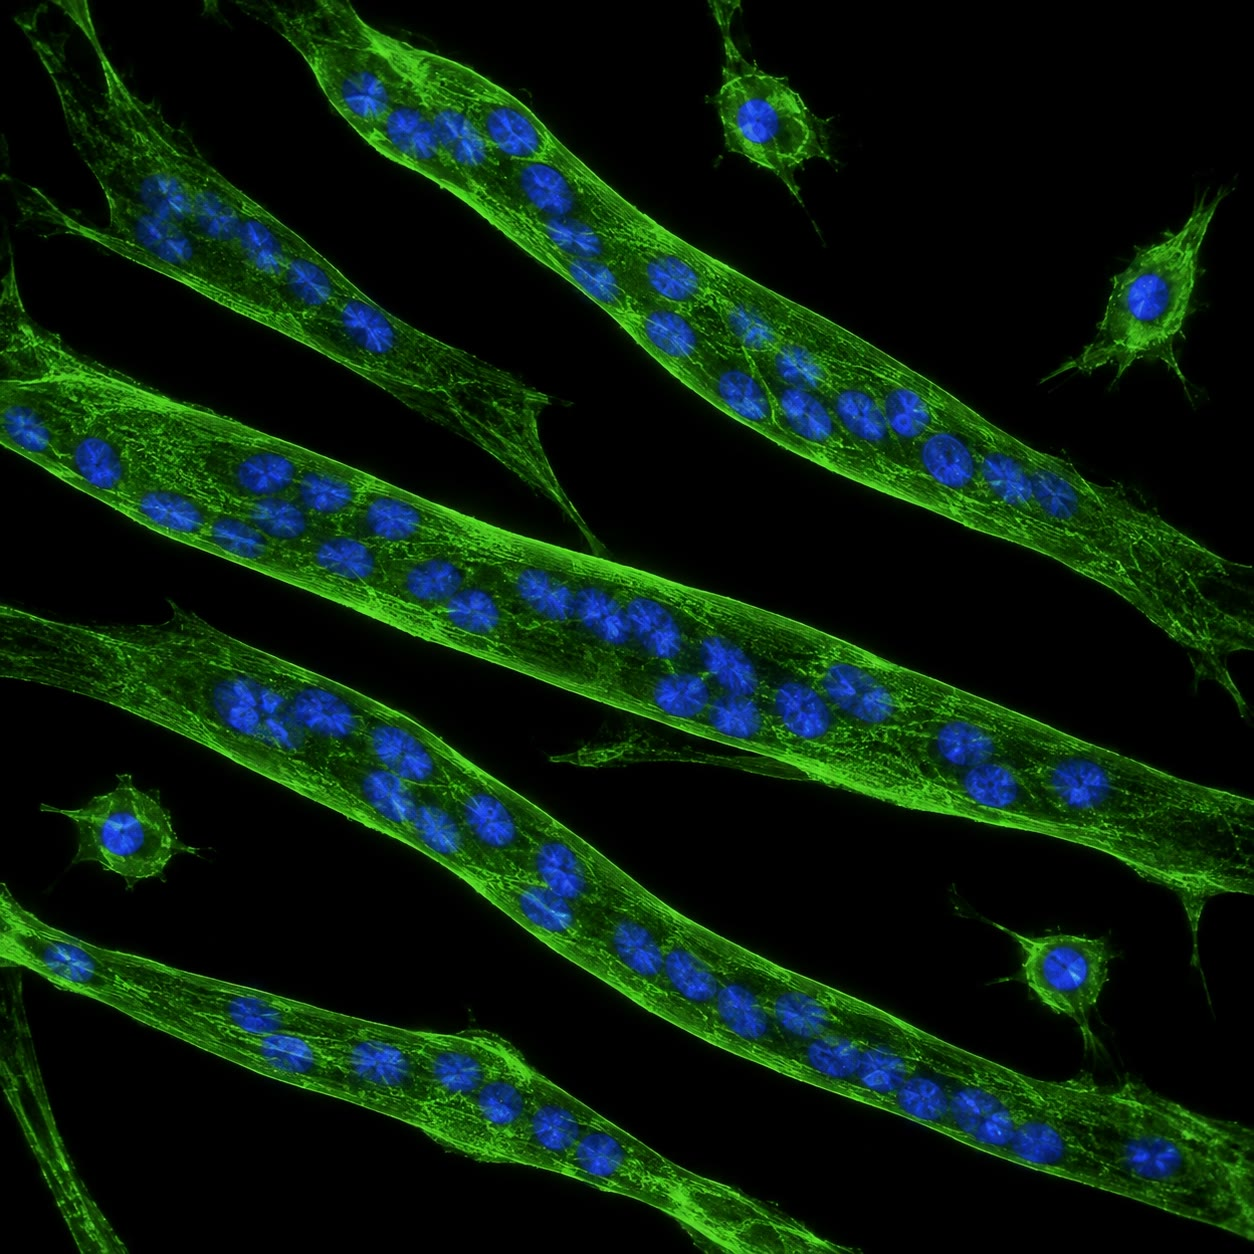
\includegraphics[width=0.44\linewidth]{images/book4/ai/b4-12-myotubes.jpg}\hspace{0.04\linewidth}
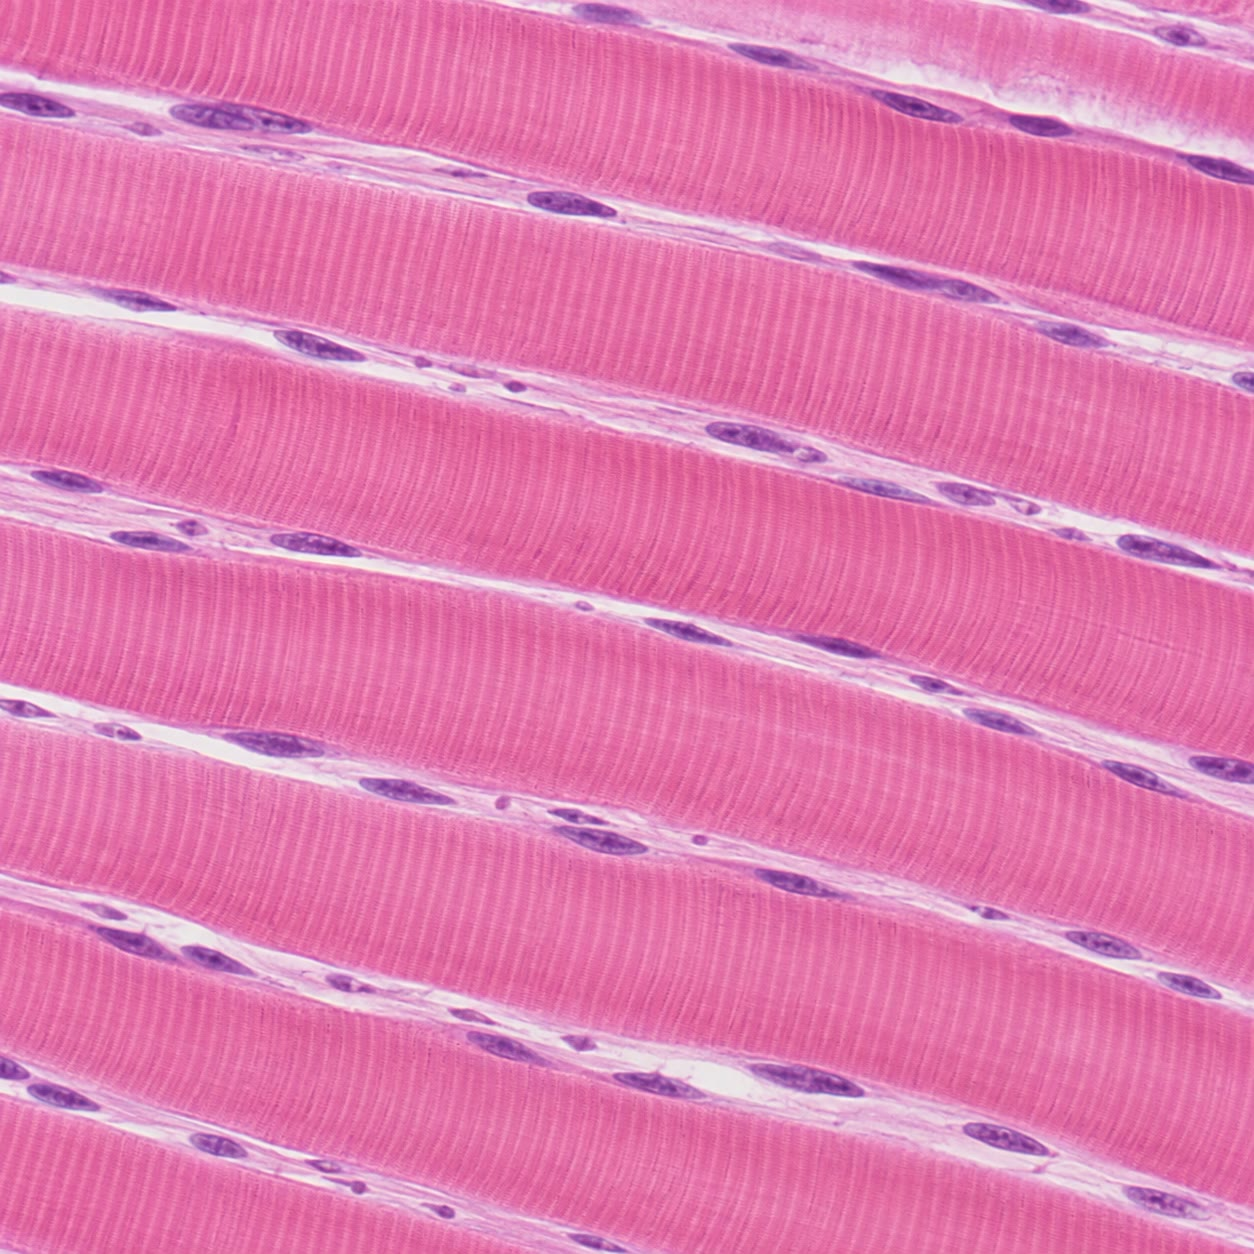
\includegraphics[width=0.44\linewidth]{images/book4/ai/b4-12-muscle-fibres.jpg}

{\small 各为融合而成的细胞，每个细胞内有一排
细胞核，旁边是尚未融合的单个\omterm{def:b2:cell-differentiation:myogenesis}{成肌细胞}。右图：
纵向视图中的成熟\omterm{def:b2:cell-differentiation:myogenesis}{肌纤维}，其横纹即
重复排列的\omterm{def:b2:cell-differentiation:fibre}{肌节}，细胞核被推至边缘。}
\end{omfigure}

\begin{proposition}[MyoD：主开关]\label{prop:b2:cell-differentiation:myod}
\index{主调控因子!MyoD}
\omterm{def:b2:cell-differentiation:myogenesis}{MyoD} 是螺旋-环-螺旋家族的\omterm{prop:b2:cell-differentiation:transcriptional}{转录因子}。它
以二聚体形式与一种广泛存在的伙伴蛋白结合，识别一段六碱基序列
即 E-box（CANNTG），位于肌肉基因的调控区
中；它招募染色质开放酶，并开启这些基因
——包括肌细胞生成素基因和 \omterm{def:b2:cell-differentiation:myogenesis}{MyoD} 自身的基因，这
正是状态得以维持的方式。其活性受门控：在分裂中的\omterm{def:b2:cell-differentiation:myogenesis}{成肌细胞}内，一个
由生长因子诱导的抑制蛋白（Id）
会隔离伙伴蛋白，使 \omterm{def:b2:cell-differentiation:myogenesis}{MyoD} 保持无活性；生长因子撤去后，Id
消失，\omterm{def:b2:cell-differentiation:myogenesis}{MyoD} 开始发挥作用。由于 \omterm{def:b2:cell-differentiation:myogenesis}{MyoD} 足以使成纤维细胞、脂肪细胞或神经细胞
获得肌肉程序，肌肉的命运在某种意义上
只取决于一个基因：成为肌肉的困难所在
不在于知道如何去做，而在于被告知要去做。
\end{proposition}
\begin{proof}[证据]
Davis、Weintraub 与 Lassar（1987）将一个从\omterm{def:b2:cell-differentiation:myogenesis}{成肌细胞}中分离的
单一 cDNA 导入培养的成纤维细胞：成纤维细胞停止分裂，
融合成\omterm{def:b2:cell-differentiation:myogenesis}{肌管}，并合成肌肉蛋白。
该基因被命名为 \omterm{def:b2:cell-differentiation:myogenesis}{MyoD}。其亲缘基因 Myf5、肌细胞生成素和 MRF4 是通过同源性
找到的；同时缺失 \omterm{def:b2:cell-differentiation:myogenesis}{MyoD} 和 Myf5 的小鼠没有\omterm{def:b2:cell-differentiation:myogenesis}{成肌细胞}，也完全没有骨骼肌，
而缺失肌细胞生成素的小鼠，
其\omterm{def:b2:cell-differentiation:myogenesis}{成肌细胞}从不融合。
\end{proof}

\begin{theorem}[自我维持的开关]\label{thm:b2:cell-differentiation:switch}
\index{双稳态}\index{正反馈!基因}
设 $m$ 为某一因子的量，该因子通过协同（S 形）响应激活自身基因，
并以速率 $k$ 降解：
\[
\frac{\mathrm{d}m}{\mathrm{d}t} = \frac{a\,m^{2}}{K^{2} + m^{2}} + b - k\,m,
\]
其中 $b$ 为较小的基础合成量。对于合适的 $a$、$b$、$K$ 与
$k$，该方程有\emph{两个}稳定的稳态：一个为接近 $b/k$ 的低值态，
另一个为接近 $a/k$ 的高值态，二者之间由一个不稳定的
阈值隔开：细胞是\emph{\omterm{thm:b2:cell-differentiation:switch}{双稳态}}的。一个短暂的诱导信号
若使 $m$ 越过阈值，就会使细胞进入
高值态，且信号消失后仍保持该状态；低于阈值时，细胞回到低值态。
这是由反馈回路构成的一种记忆，
也正因此，一旦被定向，细胞即使经过多次分裂，
在没有诱导物的情况下，仍保持其定向。
\end{theorem}
\begin{proof}
稳态满足 $k m = a m^{2}/(K^{2} + m^{2}) + b$。右侧
为从 $b$ 升至 $a + b$ 的 S 形曲线；左侧为
过原点、斜率为 $k$ 的直线。当 $b/k < K$ 且 $k$ 足够小、
使直线与 S 形曲线的陡峭部分相交时，两条曲线共有三个交点：
分别位于 $m_{\text{低}} \approx b/k$ 处，
在中间点 $m_{\text{u}}$ 处，以及位于 $m_{\text{高}} \approx (a +
b)/k$。稳定性：在 $m_{\text{低}}$ 以下，合成超过降解，
$m$ 上升；在 $m_{\text{低}}$ 与 $m_{\text{u}}$ 之间，降解超过合成，
$m$ 回落；在 $m_{\text{u}}$ 与
$m_{\text{高}}$ 之间，合成超过降解，$m$ 升至
$m_{\text{高}}$；高于它时，$m$ 回落至 $m_{\text{高}}$。
由此可知，两侧两个稳态稳定，中间一个不稳定，
即为阈值。
\end{proof}

\begin{omfigure}
\begin{tikzpicture}
\begin{axis}[
  width=0.74\linewidth, height=5.8cm,
  axis x line=bottom, axis y line=left,
  xmin=0, xmax=4, ymin=0, ymax=1.3,
  xlabel={因子水平 $m$（相对）}, ylabel={速率},
  xlabel style={font=\small, at={(axis description cs:0.5,-0.12)}, anchor=north},
  ylabel style={font=\small},
  tick label style={font=\small}, xtick={0,1,2,3,4}, ytick={0,0.5,1},
  legend style={font=\scriptsize, at={(0.03,0.97)}, anchor=north west, draw=none},
  clip=false,
]
\addplot[very thick, omDef, domain=0:4, samples=100] {x^2/(1+x^2) + 0.02};
\addlegendentry{合成：$a m^2/(K^2 + m^2) + b$}
\addplot[very thick, omThm, domain=0:3.2, samples=2] {0.4*x};
\addlegendentry{降解：$k m$}
\fill[omDef] (axis cs:0.055,0.022) circle (2pt); \draw[gray] (axis cs:0.08,0.04) -- (axis cs:0.33,0.42); \node[font=\scriptsize, anchor=west] at (axis cs:0.35,0.45) {关};
\draw[gray, thick] (axis cs:0.41,0.164) circle (2pt); \node[font=\scriptsize, anchor=west] at (axis cs:0.55,0.10) {阈值};
\fill[omDef] (axis cs:2.1,0.84) circle (2pt); \node[font=\scriptsize, anchor=north] at (axis cs:2.1,0.78) {开};
\end{axis}
\end{tikzpicture}

{\small \omterm{thm:b2:cell-differentiation:switch}{双稳态}开关（$a = 1$，$K = 1$，$b = 0.02$，$k = 0.4$）。
合成（S 形曲线）与降解（直线）相交三次：两个稳态，即关与开，
二者之间为一个不稳定的阈值。
使 $m$ 越过阈值的信号，会使细胞
永久地进入开态。}
\end{omfigure}

\section{成熟细胞}

\begin{definition}[肌纤维]\label{def:b2:cell-differentiation:fibre}
\index{肌节}\index{肌原纤维}\index{肌质网}\index{横小管}
骨骼\omterm{def:b2:cell-differentiation:myogenesis}{肌纤维}是一个直径为 \qtyrange{10}{100}{\micro m} 的圆柱形细胞，
长可达数十厘米，外包
\emph{肌膜}，紧贴其内侧排列着数百个细胞核。其
内部充满平行排列的\emph{肌原纤维}，每条肌原纤维为一串
\emph{肌节}串接而成，每个长 \qty{2.5}{\micro m}：两条 Z 盘之间，
肌动蛋白细丝（含原肌球蛋白和肌钙蛋白）锚定于
Z 盘处，与固定于
中央的肌球蛋白粗丝相互穿插，其重叠模式形成横纹。每条
肌原纤维周围缠绕着网状的\emph{肌质网}，用以储存钙；
\emph{横小管}为肌膜的内陷，横穿肌原纤维之间，
将电信号由表面传入内部。
线粒体充满其余空隙，细胞质中
储有糖原、磷酸肌酸，红\omterm{def:b2:cell-differentiation:myogenesis}{肌纤维}中还含有
肌红蛋白。细胞的构造只为一件事——按指令收缩，
——而执行该指令的机制
见\cref{ch:b2:muscle-movement}。
\end{definition}

\begin{omfigure}
\begin{tikzpicture}[every node/.style={font=\scriptsize}]
  % a stretch of myofibril with two sarcomeres
  \foreach \s in {0,4.4} {
    \begin{scope}[xshift=\s cm]
      \draw[very thick, omThm] (0,-1.1) -- (0,1.1);
      \foreach \y in {-0.9,-0.5,-0.1,0.3,0.7} { \draw[thick, omDef] (0,\y) -- (1.6,\y); \draw[thick, omDef] (4.4,\y) -- (2.8,\y); }
      \foreach \y in {-0.7,-0.3,0.1,0.5,0.9} { \draw[line width=3pt, omExo!80!black] (1.0,\y) -- (3.4,\y); }
      \draw[gray] (2.2,-1.1) -- (2.2,1.1);
    \end{scope}
  }
  \draw[very thick, omThm] (8.8,-1.1) -- (8.8,1.1);
  \node[omThm, below] at (0,-1.15) {Z 盘};
  \node[omThm, below] at (4.4,-1.15) {Z 盘};
  \node[omThm, below] at (8.8,-1.15) {Z 盘};
  \node[omDef, above] at (0.8,1.15) {细肌丝（肌动蛋白）};
  \node[omExo!80!black, above] at (6.6,1.15) {粗肌丝（肌球蛋白）};
  \node[gray, below] at (2.2,-1.15) {M 线};
  \draw[<->] (0,1.9) -- (4.4,1.9); \node[above] at (2.2,1.9) {一个肌节，\qty{2.5}{\micro m}};
  \draw[<->] (5.4,-1.6) -- (7.8,-1.6); \node[below] at (6.6,-1.6) {A 带（暗带）};
  \draw[<->] (7.8,-1.6) -- (9.8,-1.6); \node[below] at (8.8,-1.6) {I 带（明带）};
\end{tikzpicture}

{\small \omterm{def:b2:cell-differentiation:fibre}{肌原纤维}中的两个\omterm{def:b2:cell-differentiation:fibre}{肌节}：细肌动蛋白丝锚定于
Z 盘处，与肌球蛋白粗丝相互穿插，后者以
M 线为中心。其重叠形成暗的 A 带与明的 I 带，
构成横纹。}
\end{omfigure}

\begin{proposition}[纤维类型]\label{prop:b2:cell-differentiation:types}
\index{肌纤维类型}
肌肉由多种纤维类型混合而成，其类型一部分由\omterm{def:b2:cell-differentiation:myogenesis}{成肌细胞}
谱系决定，另一部分由支配该纤维的神经决定。
\emph{慢氧化型}（I 型）纤维含慢肌球蛋白、
大量线粒体和毛细血管，并含肌红蛋白——呈红色，耐疲劳，
适于维持姿势和持久运动。\emph{快糖酵解型}（IIx 型）
纤维含快肌球蛋白、少量线粒体、大量糖原——
呈白色，力量大，一分钟内即疲劳。\emph{快氧化型}
（IIa 型）纤维介于两者之间。短跑运动员的小腿以快\omterm{def:b2:cell-differentiation:myogenesis}{肌纤维}为主，
马拉松运动员的则以慢\omterm{def:b2:cell-differentiation:myogenesis}{肌纤维}为主，两者的比例可以遗传；
但类型并非固定不变：用慢神经去支配快肌，
或经数月耐力训练，纤维都会转向慢肌类型，
因为神经冲动的模式
会切换调控肌球蛋白同工型及线粒体
生物发生的基因。已\omterm{def:b2:cell-differentiation:differentiation}{分化}的细胞保持其\omterm{def:b2:cell-differentiation:myogenesis}{肌纤维}的身份，
却会依使用情况调整自身程序。
\end{proposition}

\begin{example}[生长与修复]\label{ex:b2:cell-differentiation:satellite}
成年肌肉的生长并非靠增加纤维数量，而是靠纤维增粗：
训练使每条纤维增加\omterm{def:b2:cell-differentiation:fibre}{肌原纤维}，\emph{卫星
细胞}融入其中，为变大的细胞质补充所需的额外细胞核。
受伤后，同样的细胞分裂，重新表达 \omterm{def:b2:cell-differentiation:myogenesis}{MyoD}，
融合并在数周内重建受损节段——即在成体中重新运行胚胎期的
程序。在肌营养不良症中，纤维
缺乏抗肌萎缩蛋白，该蛋白将\omterm{def:b2:cell-differentiation:fibre}{肌原纤维}与
肌膜相连，纤维在收缩时撕裂；卫星细胞
反复修复，直到数年后其储备耗尽，
纤维状组织取代了肌肉。
\end{example}

\begin{omfigure}
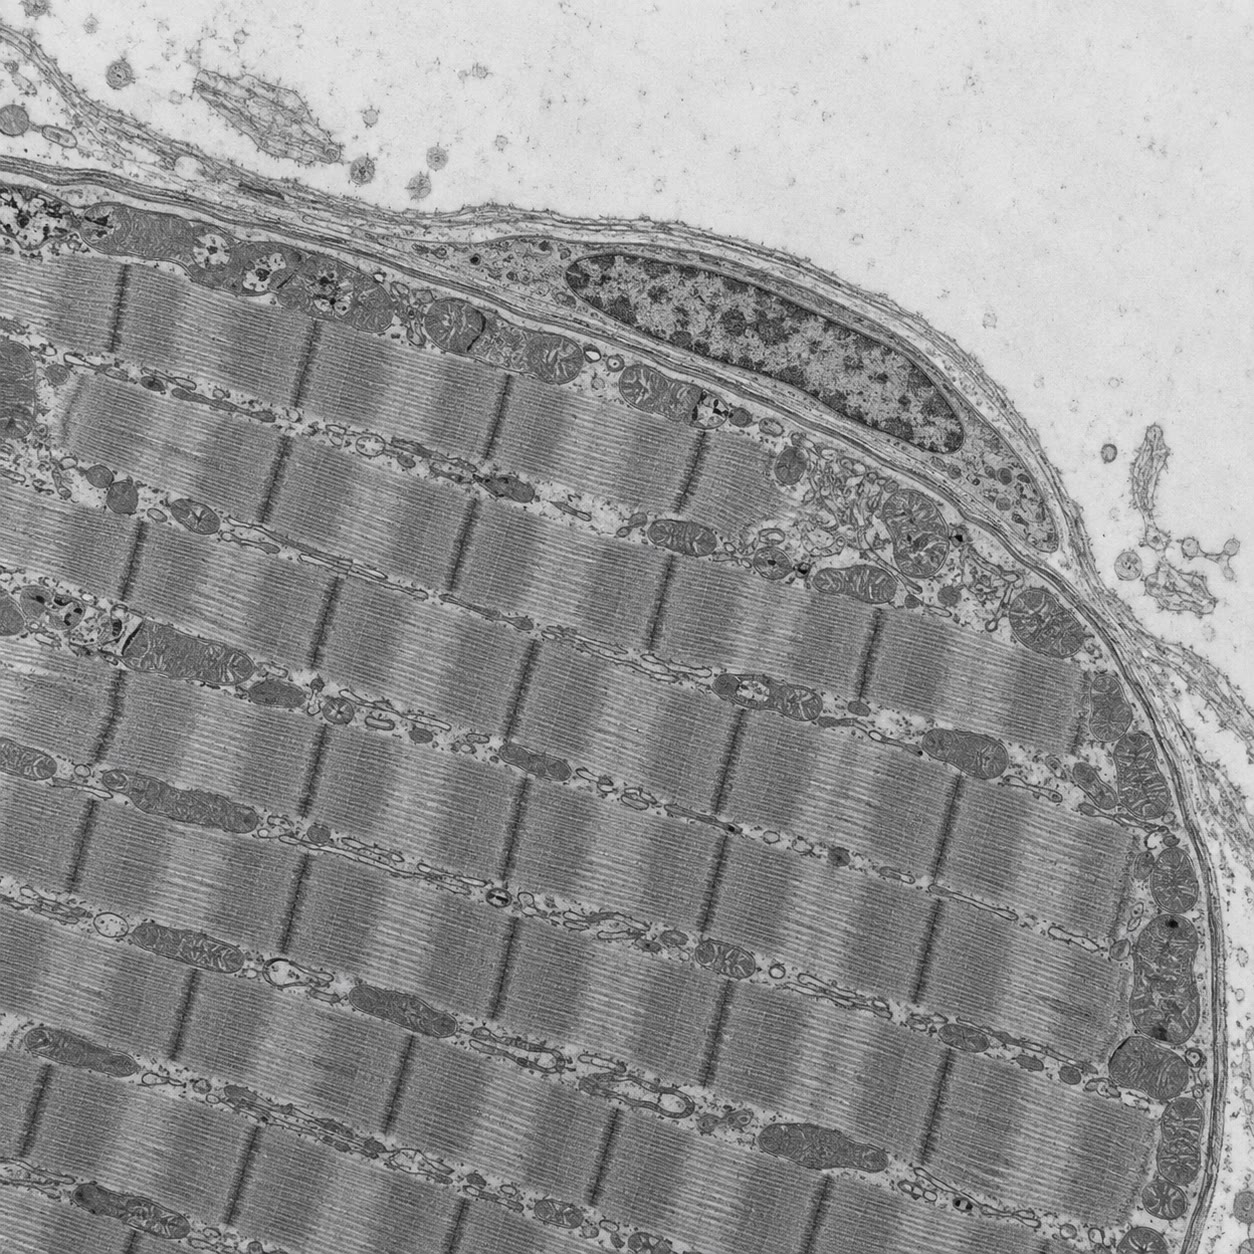
\includegraphics[width=0.42\linewidth]{images/book4/ai/b4-12-satellite-cell-tem.jpg}

{\small 电子显微镜下的卫星细胞：一个小的单核细胞，
位于\omterm{def:b2:cell-differentiation:myogenesis}{肌纤维}的膜与
其基膜之间——即纤维的\omterm{def:b2:cell-differentiation:myogenesis}{成肌细胞}储备库。}
\end{omfigure}

\section{练习}

\begin{exercise}[$\star$]\label{exo:b2:cell-differentiation:1}
定义\omterm{def:b2:cell-differentiation:differentiation}{分化}、决定与\omterm{def:b2:cell-differentiation:differentiation}{潜能}，并将
受精卵、\omterm{def:b2:mammal-reproduction:implantation}{内细胞团}细胞、卫星细胞与\omterm{def:b2:cell-differentiation:myogenesis}{肌纤维}
按\omterm{def:b2:cell-differentiation:differentiation}{潜能}高低排列。
\end{exercise}

\begin{exercise}[$\star$]\label{exo:b2:cell-differentiation:2}
列出从\omterm{prop:b2:vertebrate-development:neurulation}{体节}细胞到\omterm{def:b2:cell-differentiation:myogenesis}{肌纤维}的肌发生各步骤，
并写出每一步表达的\omterm{prop:b2:cell-differentiation:transcriptional}{转录因子}。
\end{exercise}

\begin{exercise}[$\star$]\label{exo:b2:cell-differentiation:3}
格登的核移植实验说明了什么，又未说明什么？
\end{exercise}

\begin{exercise}[$\star$]\label{exo:b2:cell-differentiation:4}
写出\omterm{def:b2:cell-differentiation:fibre}{肌节}的各组成部分，并说明
纤维缩短时哪些部分移动，哪些不移动。
\end{exercise}

\begin{exercise}[$\star\star$]\label{exo:b2:cell-differentiation:5}
一条长 \qty{20}{cm} 的纤维，\omterm{def:b2:cell-differentiation:fibre}{肌节}长 \qty{2.5}{\micro m}，
沿其长度每隔 \qty{25}{\micro m} 有一个细胞核。问：
串联的\omterm{def:b2:cell-differentiation:fibre}{肌节}有多少个，细胞核有多少个？该纤维由多少个\omterm{def:b2:cell-differentiation:myogenesis}{成肌细胞}
融合而成？
\end{exercise}

\begin{exercise}[$\star\star$]\label{exo:b2:cell-differentiation:6}
利用抑制剂 Id，解释\omterm{def:b2:cell-differentiation:myogenesis}{成肌细胞}在 FGF 存在时
为何不发生融合，
并预测经改造而组成型表达 Id 的\omterm{def:b2:cell-differentiation:myogenesis}{成肌细胞}会发生什么。
\end{exercise}

\begin{exercise}[$\star\star$]\label{exo:b2:cell-differentiation:7}
在开关模型中，取 $a = 1$，$K = 1$，$b = 0.02$，$k = 0.4$，
代入验证 $m = 2.1$ 接近稳态，
近似求出低稳态，并说明一个
其 $m$ 被短暂提高到 $1$ 后任其自然的细胞会发生什么。
\end{exercise}

\begin{exercise}[$\star\star$]\label{exo:b2:cell-differentiation:8}
在同一模型中，$k$ 提高到 $0.6$（该因子降解得更快）。用图解法或数值方法说明高稳态
消失。对 \omterm{def:b2:cell-differentiation:myogenesis}{MyoD} 失稳的细胞，
这一结果
预示着什么？
\end{exercise}

\begin{exercise}[$\star\star$]\label{exo:b2:cell-differentiation:9}
预测下列小鼠的\omterm{def:b2:meiosis-heredity:vocabulary}{表型}：(a) 同时缺失 \omterm{def:b2:cell-differentiation:myogenesis}{MyoD} 与 Myf5 的小鼠，
(b) 仅缺失肌细胞生成素的小鼠，(c) 仅缺失 \omterm{def:b2:cell-differentiation:myogenesis}{MyoD} 的小鼠。为何 (c) 几乎正常？
\end{exercise}

\begin{exercise}[$\star\star\star$]\label{exo:b2:cell-differentiation:10}
转染 \omterm{def:b2:cell-differentiation:myogenesis}{MyoD} 的成纤维细胞会形成\omterm{def:b2:cell-differentiation:myogenesis}{肌管}，而转染 \omterm{def:b2:cell-differentiation:myogenesis}{MyoD} 的肝细胞
则不会。请提出一种涉及染色质与\omterm{def:b2:vertebrate-development:induction}{感受态}的解释，
并设计一个实验加以检验。
\end{exercise}

\begin{exercise}[$\star\star\star$]\label{exo:b2:cell-differentiation:11}
耐力训练可使快\omterm{def:b2:cell-differentiation:myogenesis}{肌纤维}向慢\omterm{def:b2:cell-differentiation:myogenesis}{肌纤维}转化，而
不改变其基因组。请从基因表达角度解释神经放电模式
如何做到这一点，以及这些纤维为何仍
保持骨骼肌，而绝不会变成例如软骨。
\end{exercise}

\begin{exercise}[$\star\star\star$]\label{exo:b2:cell-differentiation:12}
“已\omterm{def:b2:cell-differentiation:differentiation}{分化}的细胞借助回路而非
\omterm{def:b2:genome-diversification:mutation}{突变}记住自己是什么。”请结合\omterm{thm:b2:cell-differentiation:switch}{双稳态}开关、染色质，以及
格登与山中伸弥的重置是可能的，但
效率低下。请展开讨论。
\end{exercise}

\section{问题：肌肉的构建与修复}

\begin{problem}[{周末问题——追踪一块肌肉从体节发育为
纤维并经历损伤的过程：成肌细胞、融合与细胞核的数目，
双稳态开关的分析，修复时间的确定，训练的定量化，
最后落在纤维的细胞核数、
开关阈值与修复时间}]
\label{pb:b2:cell-differentiation:1}
成年人的一块大腿肌有 \num{500000} 根纤维，每根
长 \qty{20}{cm}，直径 \qty{60}{\micro m}，每
\qty{25}{\micro m} 长度内有一个细胞核；\omterm{def:b2:cell-differentiation:fibre}{肌节}长为
\qty{2.5}{\micro m}。胚胎\omterm{def:b2:cell-differentiation:myogenesis}{成肌细胞}每 \qty{12}{h} 分裂一次，
前提是 FGF 存在。开关模型：$a = 1$，$K = 1$，$b = 0.02$，$k
= 0.4$。一次损伤破坏了每根纤维 \qty{10}{\%} 的
长度后，受伤节段的卫星细胞（\num{4} 个
每毫米纤维）每 \qty{18}{h} 分裂一段时间，随后融合。

\medskip
\noindent\textbf{第一部分——纤维。}
\begin{enumerate}
  \item 计算一根纤维中串联排列的\omterm{def:b2:cell-differentiation:fibre}{肌节}数目，以及
        细胞核数目。
  \item 形成一根纤维共有多少个\omterm{def:b2:cell-differentiation:myogenesis}{成肌细胞}融合？整块肌肉呢？
  \item 计算一根纤维以及整块肌肉的体积（以
        升为单位）。
  \item 估算一个细胞核所服务的细胞质体积，并
        与体积为 \qty{2000}{\micro m^3} 的普通细胞作比较。
  \item 为何成熟纤维中的细胞核位于外周？
  \item 该肌肉的\omterm{def:b2:cell-differentiation:myogenesis}{成肌细胞}由 \num{2000} 个\omterm{prop:b2:vertebrate-development:neurulation}{体节}
        细胞衍生而来。它们需要多少次倍增，以及多少天，
        才能达到第 2 题所求的数目？
\end{enumerate}

\medskip
\noindent\textbf{第二部分——开关。}
\begin{enumerate}[resume]
  \item 写出稳态条件，并证明 $m \approx
        0.055$ 满足该条件。
  \item 证明 $m \approx 2.1$ 满足该条件。
  \item 证明在 $m = 0.41$ 附近存在第三个解，并
        由 $\mathrm{d}m/\mathrm{d}t$ 在两侧的符号说明
        该解不稳定。
  \item 一次诱导物脉冲使 $m$ 升至 $0.6$，另一次升至 $0.3$。
        各细胞的命运如何？
  \item 一次\omterm{def:b2:genome-diversification:mutation}{突变}使基础合成 $b$ 升至 $0.4$。
        证明低稳态消失。该细胞将如何？
  \item 说明该模型如何解释定向决定在
        细胞分裂后仍得以保持，以及每次分裂时 $m$ 须满足什么条件。
\end{enumerate}

\medskip
\noindent\textbf{第三部分——修复。}
\begin{enumerate}[resume]
  \item 一根纤维携带多少个卫星细胞，损伤后
        必须补充多少个细胞核？
  \item 卫星细胞需经历多少次倍增，才能
        提供这些细胞核，所需时间多长？
  \item 与观察到的两到三周修复时间相比较，并
        说明这段时间还包括哪些内容。
  \item 为何卫星细胞在融合前必须重新表达 \omterm{def:b2:cell-differentiation:myogenesis}{MyoD}，
        且为何必须先停止分裂？
  \item 每一轮修复都会消耗一部分卫星细胞。若
        每次损伤后池中数量下降 \qty{5}{\%}，经过多少次损伤
        池中数量才减半？
  \item 经过二十次此类损伤后，每根纤维
        还剩多少个卫星细胞？
  \item 营养不良性肌肉的纤维在每次收缩时都会撕裂。
        解释为何这种肌肉数年后会被纤维组织取代。
\end{enumerate}

\medskip
\noindent\textbf{第四部分——训练。}
\begin{enumerate}[resume]
  \item 训练使每根纤维增粗至 \qty{80}{\micro m}。纤维体积
        增长为原来的多少倍？卫星细胞需额外提供多少个细胞核，若
        保持第 4 题的比例
        不变？
  \item 计算该肌肉的新体积。
  \item 耐力训练使 \qty{30}{\%} 的快\omterm{def:b2:cell-differentiation:myogenesis}{肌纤维}
        转变为慢\omterm{def:b2:cell-differentiation:myogenesis}{肌纤维}。这些纤维中哪些已经改变，哪些
        未改变？
  \item 解释成年肌肉为何通过纤维增粗而增大，
        而不是增加纤维数目，这里利用了纤维
        不分裂这一事实。
  \item 某药物阻断卫星细胞的融合。预测该肌肉
        对训练和损伤的反应。
  \item 给出结果：纤维的细胞核数、开关阈值，
        以及卫星细胞为修复提供细胞核所需的
        时间。
\end{enumerate}
\end{problem}
